\chapter{User experience} \label{cha:userexperience}

\section{Basis functionaliteit} \label{sec:basis}
\projectname\ maakt gebruik van vision om de bewegingen van de gebruiker te registreren. De gebruiker moet daarom gemakkelijk de applicatie kunnen gebruiken met zijn/haar handen. De knoppen moeten genoeg van elkaar verspreid staan zodat er geen onhandige situaties ontstaan waarbij de gebruiker per ongeluk knoppen indrukt.\\
Dit wordt verder behandeld in \cref{sec:layout} \nameref{sec:layout}. In \cref{fig:statemachine1} staat weergegeven hoe de gebruiker navigeert door de applicatie.

\begin{figure}[h]
	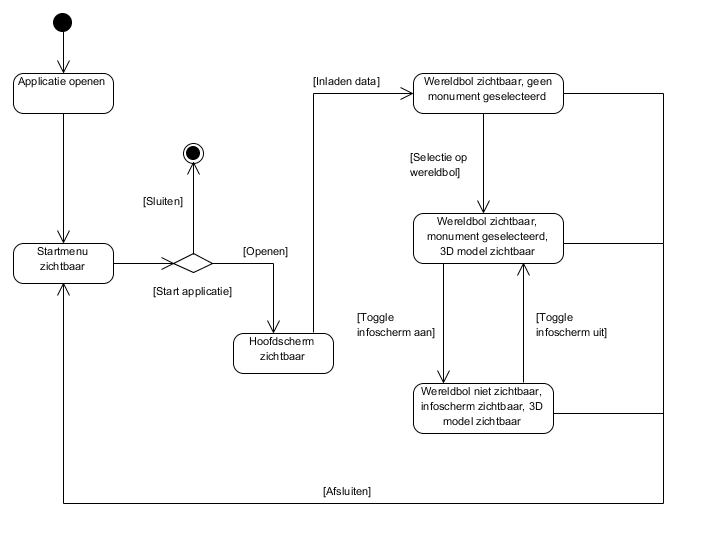
\includegraphics[width=130mm]{figs/state_machine1.png}
	\caption{State Machine diagram userflow}
	\label{fig:statemachine1}
\end{figure}


\newpage
\section{Opstelling} \label{sec:setup}
\begin{figure}[h]
	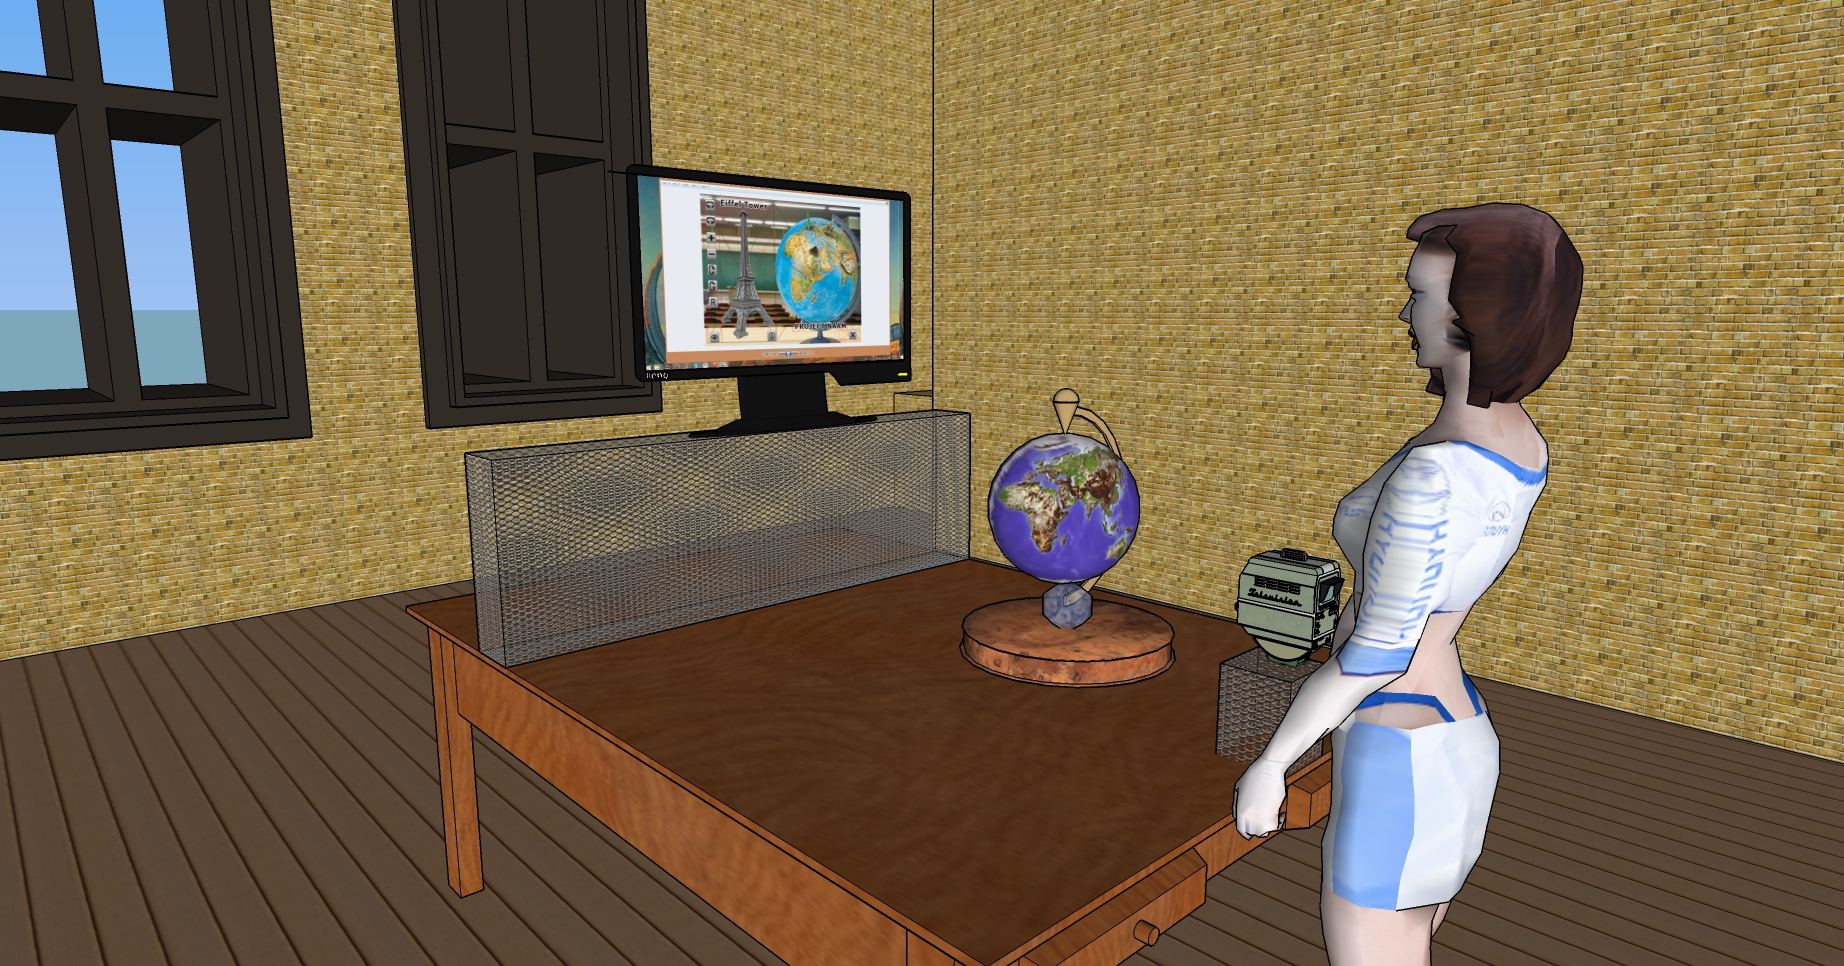
\includegraphics[width=130mm]{figs/screen1.jpg}
	\caption{Fysieke opstelling}
	\label{fig:screen1}
\end{figure}

\begin{figure}[h]
	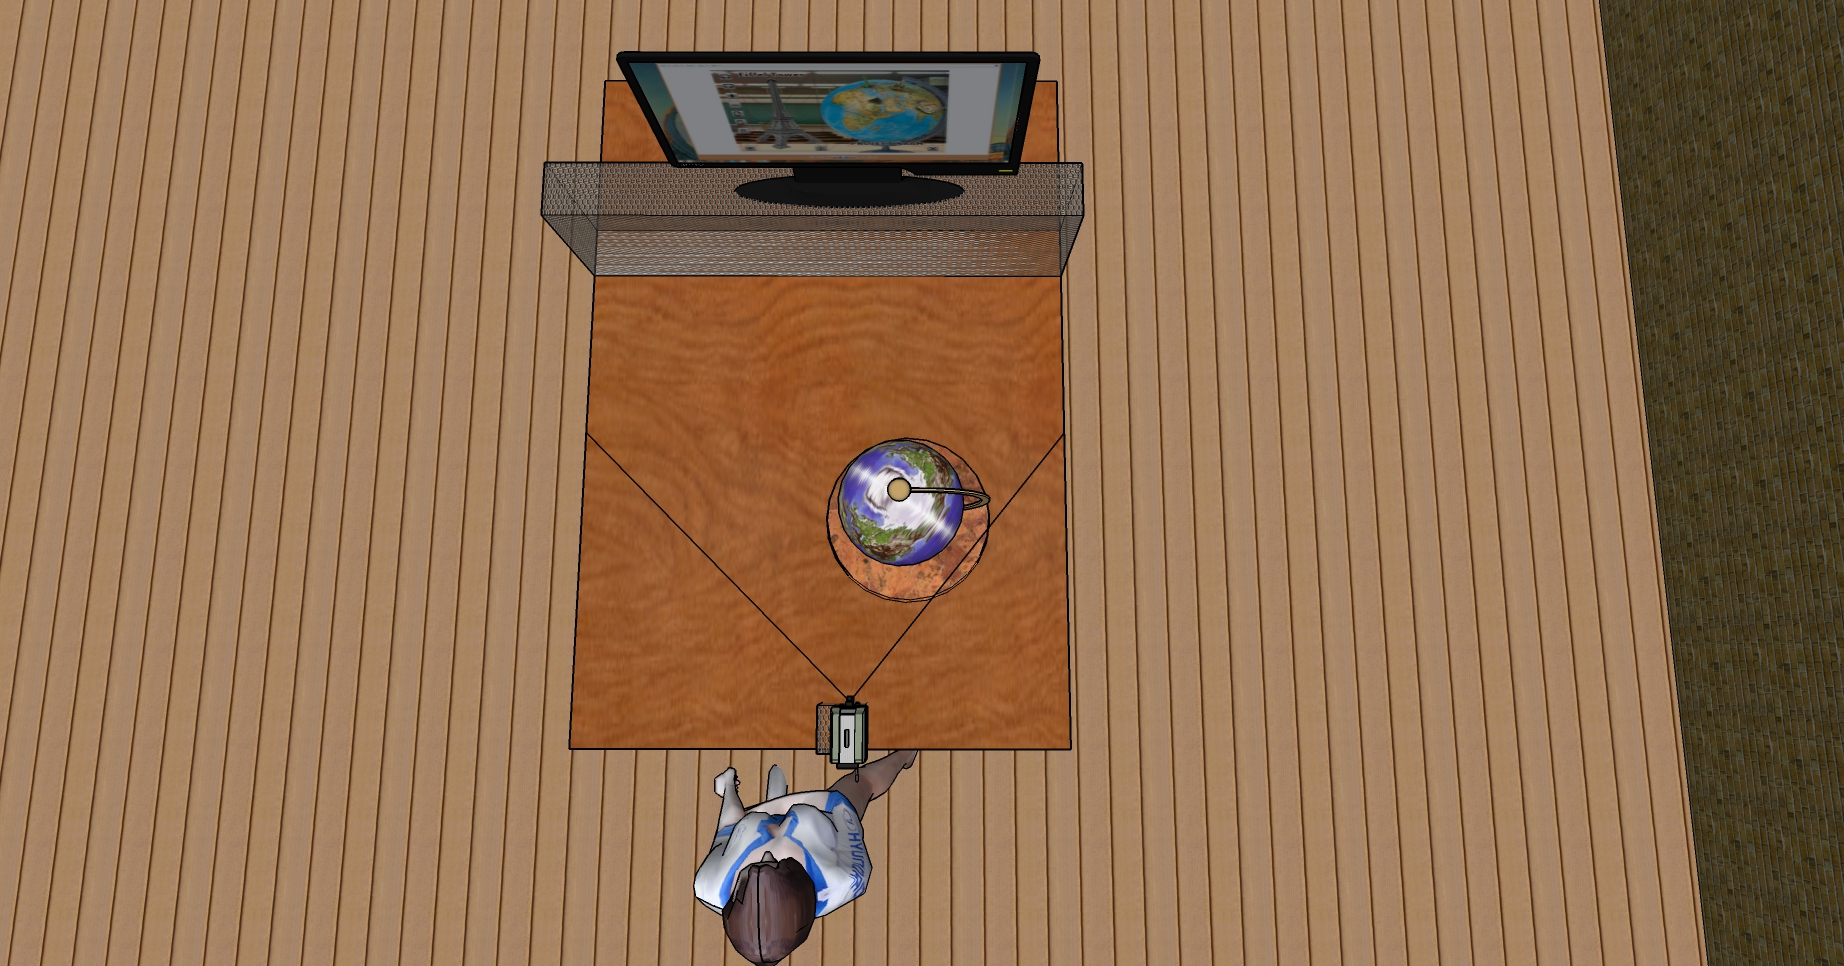
\includegraphics[width=130mm]{figs/screen2.jpg}
	\caption{Fysieke opstelling (topview)}
	\label{fig:screen2}
\end{figure}

Deze concept schetsen (\cref{fig:screen1} en \cref{fig:screen2}) geven het basis idee weer van hoe het gehele product zou moeten worden opgesteld. De camera staat op correcte hoogte om de wereldbol goed weer te geven, maar kan hinderlijk worden ervaren door de gebruiker. De wereldbol staat binnen armlengte van de gebruiker. De camera registreerd de rotatie van de wereldbol en de handen van de gebruiker. Op een computerscherm wordt de applicatie weergegeven, dit scherm wordt verhoogd naar ooghoogte van de gebruiker. Het gehele product moet ergonomisch worden ingericht, nader onderzoek zal worden gedaan naar exacte afmetingen. 

\newpage
\section{Layout} \label{sec:layout}
\begin{figure}[h]
	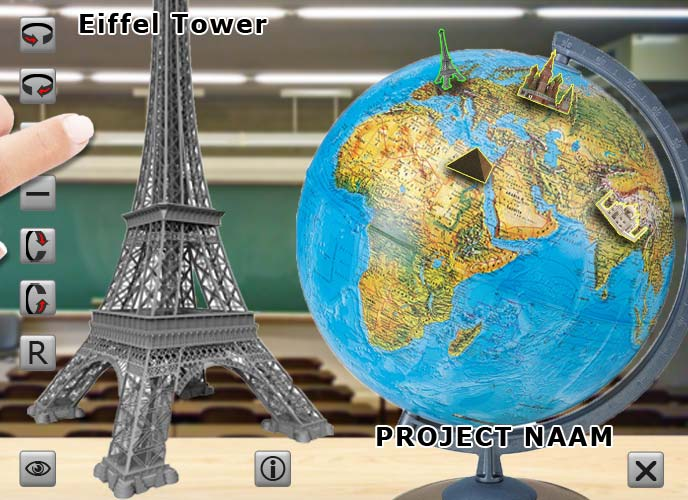
\includegraphics[width=100mm]{figs/userexp1.jpg}
	\caption{Gebruiker interactie}
	\label{fig:userexp1}
\end{figure}

De opstelling van de camera vereist van de gebruiker om zijn/haar handen om de camera heen te bewegen om zodanig de knoppen te kunnen bedienen. Deze manier van navigeren is niet geheel efficient en kan in de praktijk als onprettig worden ervaren. Om dit zoveel tegen te gaan zijn een aantal voorbereidingen getroffen.
\subsection{Knoppen margin} \label{subsec:margin}
De ruimte tussen knoppen is vergroot, zodat de kans dat de gebruiker de verkeerde knoppen indrukt verkleint. De knoppen hebben ook een offset vanaf de rand van het scherm, dit zorgt ervoor dat de gebruiker enigzins zijn/haar hand kan zien bewegen en een inschatting kan maken waar zijn/haar exacte locatie is op het scherm.
\subsection{Camera afstand} \label{subsec:cameraafstand}
De brandpuntafstand van de camera kan worden gekalibreerd zodat deze optimaal is voor zowel de hand van de gebruiker als de wereldbol. Aangezien de wereldbol binnen armlengte moet staan, kan de gebruiker dus ook met zijn/haar hand op dezelfde afstand houden. Dit zorgt voor optimale focus van de hand en de wereldbol.
\subsection{Functionliteiten schrappen} \label{subsec:scrap}
Als laatste oplossing worden bepaalde knoppen (en daarmee functionliteiten) van het scherm verwijderd om een optimalere gebruikersinteractie te krijgen. Het belangrijkste is dat de gebruiker gemakkelijk en ergonomisch de applicatie kan gebruiken. Dit betekent dus dat de layout zoals is weergegeven in dit document niet definitief is.